\documentclass[journal,compsoc]{IEEEtran}
\usepackage[nocompress]{cite}
\usepackage[font=normalsize,labelfont=sf,textfont=sf]{subfig}
\usepackage{graphicx}
\usepackage{arabtex}
%\usepackage{fixltx2e}
%\usepackage{stfloats}
%\usepackage{url}
\usepackage[cmex10]{amsmath}
%\usepackage{array}
%\usepackage{mdwmath}
%\usepackage{mdwtab}
%\usepackage{eqparbox}

%packages that were not copied from the IEEE template - need to check if it is valid to add them
\usepackage{amssymb}
\usepackage{multicol}
\usepackage{algorithm2e}

%TODO: make sure that all citation are before the period and not after.
%TODO: Add biography and image for me and for DR. Raid.
%TODO: Check for plagiarism in all the document.
%TODO: Read the IEEE specification again.

\begin{document}

\title{Recognition-based Segmentation of On-line Handwritten Arabic Script}


\author{George~Kour,
		Raid~Saabne}

%\markboth{Journal of \LaTeX\ Class Files,~Vol.~6, No.~1, January~2007}%
%{Shell \MakeLowercase{\textit{et al.}}: Bare Demo of IEEEtran.cls for Computer Society Journals}

\markboth{\today}{}

%\IEEEspecialpapernotice{(Invited Paper)}


\IEEEcompsoctitleabstractindextext{
\begin{abstract}
character segmentation has an integral role in many Optical Character Recognition (OCR) systems due to the fact that correctly segmented characters are likely to be recognized correctly. However, Correct and efficient segmentation of Arabic text into characters is considered to be an essential problem. The cursive and unconstrained nature of the Arabic script in both printed and handwritten forms anneals the segmentation task. The Arabic script is composed of strokes which represent a single letter, multiple connected letters or diacritics. This paper proposes a novel on-line strokes-level recognition-based segmentation technique of Arabic script. The advantage of our approach is that the most time consuming procedures are performed while the stroke is being scribed. The system consists of three stages. The first stage, which requires the most calculation effort, is performed whilst the stroke is being written and involves three main parts: 1. Preprocessing of the written stroke. 2. Over-segmentation of the written stroke using on topological and directional local features. 3. Recognition-based scoring of adjacent combinations of sub-strokes that induced by the proposed segmentation points. The second stage contains filtering of the topologically invalid segmentation points. The last stage involves several segmentation points selections algorithm which determines the best subset of segmentation points. The system has been designed and tested using the ADAB Database. Promising results were obtained without using context help.
\end{abstract}
\begin{IEEEkeywords}
Arabic Handwriting Recognition, Arabic Script Segmentation, Arabic Strokes Segmentation, On-line Text Recognition
\end{IEEEkeywords}
}
\maketitle

\IEEEdisplaynotcompsoctitleabstractindextext

\section{Introduction}
\date
\IEEEPARstart{H}{andwriting} remains the most used mean of communication and recording of information in the daily life. Therefore, a growing interest in the on-line character recognition field has taken place in the recent years. Handwriting recognition can be categorized into two main fields: off-line and on-line. In the off-line script recognition, a digital image containing text is fed to the computers and the system attempts to convert the spatial representation of the letters into digital symbols \cite{al2011online}. On the contrary, on-line handwriting recognition refers to the situation where the recognition is performed concurrently to the writing process. Approaches for script recognition are usually classified into two types: 1.The holistic approach \cite{biadsy2011segmentation} and 2.the analytic approach \cite{abdulla2008off, sari2002off, Dinges2011, elanwar2012unconstrained}. The holistic approach considers the global properties of the written text while the analytic approach involves segmentation and classification of each part of the text.  In the holistic approach, the recognition system needs to be trained over all words in the dictionary, while it is possible for small vocabulary of words; this is not feasible for large vocabularies (20,000 words or more). Since each word is constructed from a subset of the character alphabet, it is much more efficient to classify words using the analytic approach \cite{elanwar2012unconstrained}.\\

The main motivation behind researching the field of Arabic handwriting segmentation its widespread. Although no reliable resource could be found which the exact number of people whom read and write the Arabic text, it is known that the the Arabic language is the forth most spoken language by natives after Mandarin, Spanish and English. The Arabic language contains many different dialects used for nearly all everyday speaking situations however the formal standardized language, found mostly in writing or in prepared speech, is common \emph{[add citation from Wikipedia]}.  Approximately 25 languages have adopted the Arabic writing system with some changes. Thus the ability to segment and recognize Arabic script would have a significant academic and economic impact. Nevertheless, the Arabic script recognition is at early stage in relation to the script recognition of Latin, Chinese and Kanji which has been a focus of study in the last decade and achieved an impressive recognition rates. Complexities such as cursiveness, context sensitive shapes and overlapping of the Arabic script causes the OCR of the Arabic languages much more complicated than other languages such as English and Chinese \cite{razzak2010locally}. 
Character Recognition of the Arabic script is more complicated than other languages such as English and Chinese due to complexities such as cursiveness, context sensitive shapes and overlapping. 

The reason for this is mainly the peculiarity nature of the Arabic script, lack of funds and other utilities such as text database, dictionaries, etc.\cite{zeki2011segmentation}.\\

The Arabic language is written right to left in a cursive manner in both handwritten and printed forms. Most Arabic letters has four main body shapes: Isolated, Medial, Initial and Final, while other letters have two main body shapes: Isolated and Final. An occurrence of two shapes letters inside a word will lead to a split of the body into two or more parts, called Word-Parts (WPs). Within the WP, the letters are connected in both handwritten and printed. Different letters may share the same body and only differ by additional strokes and dots named diacritics. For example the letters \RL{.h}  (Ha),\RL{j} (Jim),\RL{x} (Kha), and also the letters \RL{r} (Ra),\RL{z} (Zayn) and more.
In many cases Arabic WPs, which are connected when printed, are written in multiple strokes in handwritten form as can be seen in figure \ref{fig:kmbot}. \\

\emph{[consider adding a table of the similar body letters.]}\\

Correct segmentation of a word into letter is likely to result in a correct recognition. The other way around is also valid when it comes to recognition-based segmentation techniques, i.e. a firm recognition system improves the segmentation precision. Several segmentation approaches have been proposed in the literature for Arabic OCR. Yet, correct and efficient segmentation of Arabic text is an unmet need and considered to be a challenging and a fundamental problem even for off-line printed text. A common approach that is followed by many researchers is over-segmentation of the text and validating each such candidate segmentation point by extracting feature vectors representing the segmented parts to some classifier or rules based engine \cite{daifallah2009recognition}.\\

\emph{[talk about over and under segmentation in the general case, not specifically to the Arabic]}\\

Methods used by segmentation-based approaches can be mainly classified into two: Dissection and Recognition-Based Segmentation. Dissection techniques learn the characteristic of the segmentation point and attempt to find appropriate candidate points. For instance, local minima in the upper or lower contour is commonly used for segmenting English cursive script.\emph{[TODO:add citation]}. Other widely used feature that characterizes a segmentation point is the low slope of its local environment. The dissection of words into segments do not necessarily correspond to exactly one character per segment, however it could segment the words into components called graphemes, which are a combination of two or three letters, or a part of a letter. The relationship between graphemes and letters is applied in a later phase \emph{[TODO:add citation]}. The recognition-based techniques operate quite differently. The method includes using a moving window with a predefined width which breaks the word into many overlapping pieces without regard to its content and the attempts to classify those sub-components to find points of interest or trajectories. An iterative or parallel scanning of the words followed by a recognition method is used to search for "satisfactory" classification scoring for joint sub-components usually by generating a lattice of all or many possible combinations. The final decision is determined by the best path through the lattice. While avoiding using complex dissection methods, such techniques rely heavily on the classifier accuracy \cite{casey1996survey}. \\

In this paper we propose a novel approach which performs segmentation and recognition in the strokes level. We combine both holistic and analytic techniques for recognizing open dictionary Arabic on-line script. In section \ref{sec:related_word} we mention related studies done in the field of on-line Arabic recognition. The proposed approach is described in details in section \ref{sec:approach}. Results are shown in the section \ref{sec:results}. We present the future work we plan in section \ref{sec:future_work}.

\begin{figure}
\centering
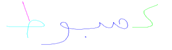
\includegraphics[width=6cm]{./figures/kmbot_color}       
\caption{The Tunisian city name kambot \RL{kmbw.t}. It contains two word parts (\RL{kmbw} and \RL{.t}). The main body of the first WP is written using three strokes: 1. The letter \RL{k-} 2. The connected letters combination \RL{-mbw} 3. The additional dot of the letter \RL{-b-}. The second WP contains only a single letter (\RL{.t}) and is written using two strokes, the main body and an additional stroke.}
\label{fig:kmbot}
\end{figure}

\section{Related Work}
\label{sec:related_word}
A rules-based system for off-line Arabic handwritten word segmentation was presented by Abdulla et al. in \cite{abdulla2008off}. Their method is based on extracting features of pixels lying on the upper contour. The freeman chain coding scheme was used to find the coordinates of the contour. After calculating the slope of the upper contour pixels, the direction of pairs of adjacent coordinate were marked by '+' or '-'. Segments were combined to formulate bigger decisive segments (DS). Then, a set of possible segmentation point are nominated from the ‘+’ marked segments. These segmentation points were evaluated using a certain rules to find the final segmentation points (FSP). The system was tested on the demo version of IFN/INIT described in \cite{pechwitz2002ifn} , and their own AHD/AUST database.\\

Randa et al. proposed a two stage word segmentation system of on-line Arabic handwritten text based on Hidden Markov Model (HMM) in \cite{elanwar2012unconstrained}. In the first stage, segmentation points were nominated by a simultaneous segmentation-recognition method using HMM. The proposed segmentation points were validated by a rules-based stage. Additional strokes were removed and not taken into consideration in both parts. The system was tested using a self-collected database (OHASD) that was described in \cite{elanwar2010ohasd}.\\

Another method described in \cite{sari2002off} by Sari el al. proposed a method for off-line Arabic Word parts segmentation based on the topological characteristics of the word contour. A contour following  algorithm was applied to achieve a smoothed sequence of the X-Y coordinates of the outer contour. Local minima were identified in the lower contour to nominate segmentation points. Then, a rules based engine was employed to identify valid segmentation points. The system was evaluated using a small database that contained 100 handwritten Arabic words sampled.\\

A segmentation based recognition approach was described by Laslo Digness et al. in \cite{Dinges2011}. Their method is based on dividing the word to smaller pieces which afterwards segmented into candidate letters and then classified into letter classes using statistical and structural features. Decisive tree were used to reduce the number of potential classes; neural networks to compute weights for all statistical features. The output of this process was used as input for a k-NN classifier to obtain the final recognition.\\

Khaled Daifallah et al. in \cite{daifallah2009recognition} proposed a method for on-line Arabic handwritten words recognition. Their method operates on the stroke level. It is based on segmentation-based recognition which contain several stages. The first stage proposes over-segmentation of the stroke. The segmentation points are selected by locating semi-horizontal lines moving from right to left. In a latter phase, a portion of the segmentation points is filtered out by applying on a certain set of rules. Then, HMM is used to classify the sub-strokes to letters using Hu feature. The candidate and its scoring letters results were used to determine the best set of segmentation points. \\

Eraqi and Abdelazeem \cite{eraqi2012new} suggested splitting the Arabic handwriting off-line data into basic graphemes based on the geometric properties. The image was skeletonized and using Douglas-Peuker lines simplification algorithm, linear piecewise linear curves were obtained. Diacritics and noise segments that often appear in the binarized image were removed. Horizontal segments were found by calculating the angle between the skeleton lines of the shape and the x-axis. Linear regression was used to find the baseline and all least fitting segmentation points filtered out. Then, a rules based procedure was applied to extract the graphemes corresponding to the final segmentation points were extracted.    

\section{Approach}
\label{sec:approach}
Our approach employs both rules-based dissection and recognition-base segmentation techniques. The main idea of is to  segment a stroke while being scribed. A stroke is a subcomponent of a WP that spans from the pen down event to the corresponding pen up event. We assume that each letter is contained entirely in a stroke, i.e. no letter span over multiple strokes. This assumption is valid for the majority of Arabic writing styles. 
A stroke is represented by a sequence of points on the 2-dimensional space, $p_{i}=(x,y)$ 
\begin{equation}
S=\{p_{i}\}_{i=1}^{n}
\end{equation}
The motivation behind this method is based on the intuition that the most basic structure that can be recognized by a human reader and thus can be segmented is the stroke which is a self contained component. Thus being able to correctly segment and recognize the content of a stroke, will vastly facilitate the Arabic script recognition problem. In this work our objective is to maximize the correct segmentation rate while maintaining low complexity and high performance of the system, rather than maximizing the recognition results. 
The proposed technique describes a general concept of ongoing strokes segmentation. The decoupling between the different components and sub-components in the system enables different alternatives techniques to be integrated easily such as dissection techniques and graphemes or letters classification. A high level visual description of the system can be seen in figure \ref{fig:system_flow}.\\

Below, a digest of the three main stages of our approach: \\

\textbf{Stage 1.} This stage is activated on every reception of a new point by from the tablet. The whole trajectory received since the last "pen down" event is preprocessed to remove noises and imperfections. The horizontal handler that joint a pair of connected Arabic letters is mostly horizontal, directed right to left and located near the baseline, thus our goal is identify this Horizontal segments and pinpoint a segmentation point, preferably, as much as close the the middle of the handler. Thus, the preprocessed stroke is investigated in an attempt to determine whether the newly acquired point represents the beginning of a new horizontal fragment or end of an horizontal fragment (HF) by calculating the slope of the local point area. If a the last point ends a HF, the medial point of the HF is nominated as a Candidate Point (CP). For each new CP is a row and a column is added to the Subsequence Scoring Matrix which contains the classification scoring of sub-strokes spanning from candidate point that spans between any two candidate points. The scoring is calculated using a letter classification system. Once the corresponding "Pen up" event occur, the system moves for the next stage.\\ 

\textbf{Stage 2.} The CP's are investigated and both invalid and redundant candidate points are filtered out. Then, a scoring correction process is invoked to adjust very high scoring for least probable candidate points using some heuristics. An example for invalid candidate point can be a point which do not reside on a HF or on a contour of a loop. Redundant candidate point happens when more than a single candidate point were nominated on the same HF  that represent joint trajectory between two connected letters.\\

\textbf{Stage 3.} At this point the scoring matrix is ready and all the bad candidate points are eliminated. Next, a collection of algorithms is employed to select the final set of segmentation points.

Detailed explanation on each stage is provided in the subsections below.

\begin{figure}
\centering
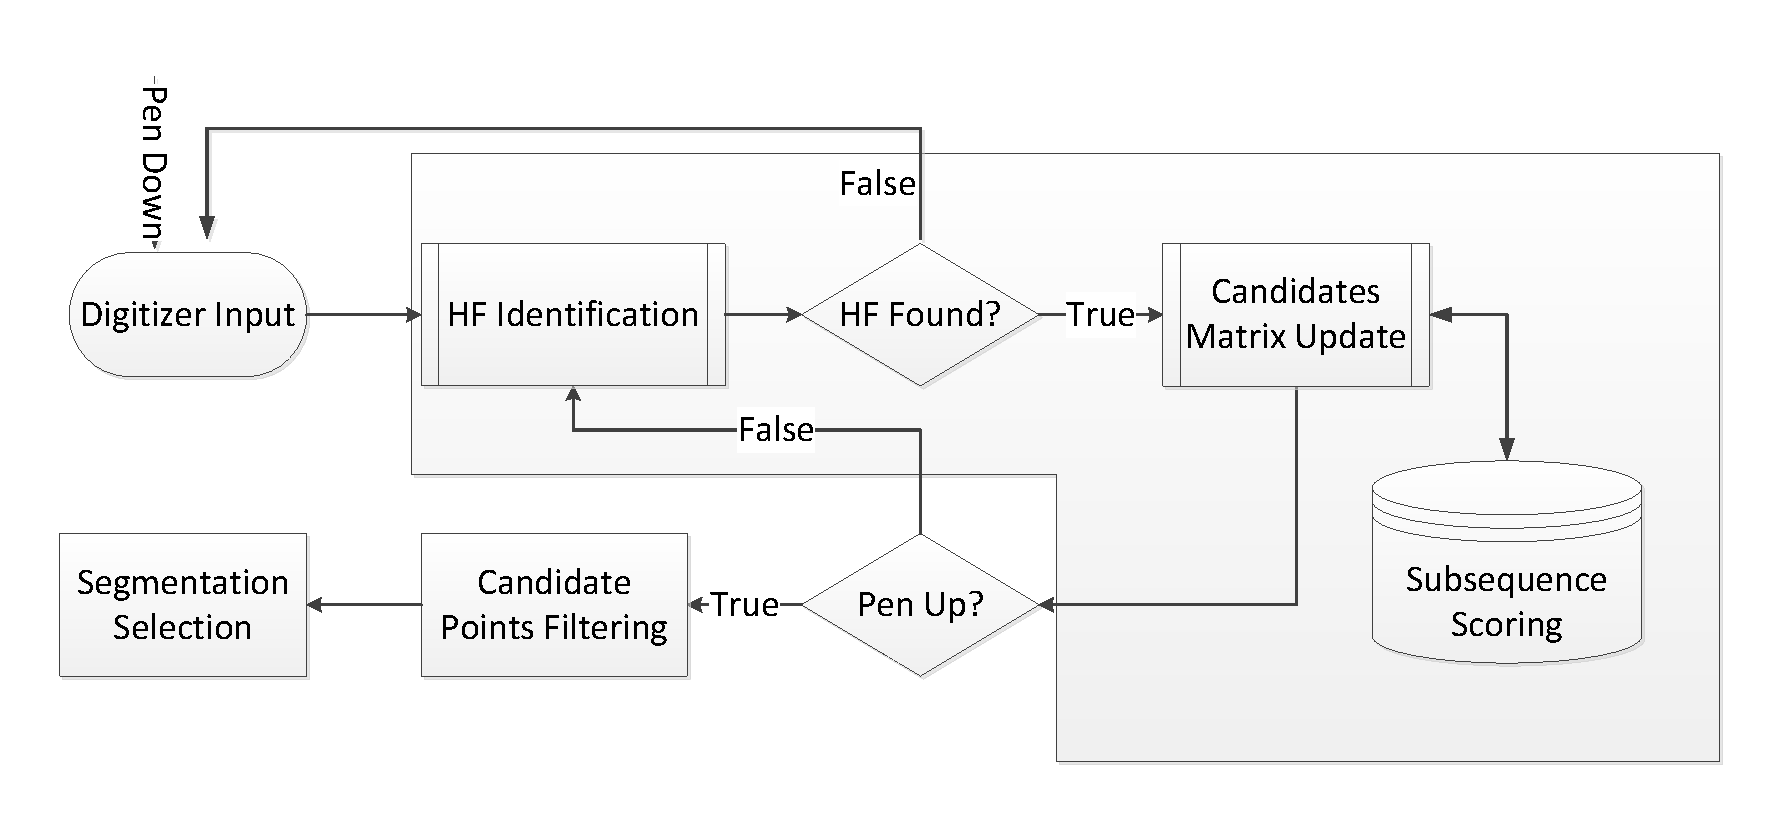
\includegraphics[width=9.5cm]{./figures/system_flow}
\caption{High level system flow. The first stage is multi-phase and contain three subcomponent. }
\label{fig:system_flow}
\end{figure}

\subsection{First Stage: Segmentation points nomination and sub-strokes scoring}
\subsubsection{Preprocessing}
\label{preprocessing}

\emph{[note that the preprocessing is not done before the HF identification process, but a lite version of it. The complete process is is done only before giving it to the classifier.]}\\

The data obtained by the digitizer is composed of points in the plane that represent the trajectory scribed by the writing instrument on the tablet surface. The data obtained is not assured to be equidistant, filtered or having a uniform structure. On the contrary, it is likely to contain noises and imperfections caused by the handwriting speed, hand vibrations, and general digitizer faultiness.   
To overcome the flaws mentioned preprocessing operations are usually applied. The preprocessing steps imposes certain uniform structure on the data to comply with the input structure required by the latter parts of the system, such that vector length, sequence bounds, etc.
Our preprocessing phase include three steps in the following order: normalization, simplification and then re-sampling.\\

\textbf{Normalization.} Size normalization is done to achieve a uniform size of the bounding box surrounding the pattern. This is done to enable the classifier to recognize the sequence pattern even when the stroke is written in different sizes. Shape similarity algorithms tend to be sensitive for nonuniform shapes size, thus this procedure is important and can be found in many approaches in the literature. The bounding box of the sequence after this procedure is $[0,1]\times[0,1]$. We include in this step also translation of the sequence's center of gravity to the origin point $[0,0]$.\\

\textbf{Simplification.} The input obtained by the digitizer may contain a large amount of noise. The noise is mainly duplication of points. In this process redundant points are filtered out and a similar sequence with fewer points is obtained. Douglas-Peucker algorithm is used and the maximum distance parameter used by the algorithm is set to be \emph{[]}. The resulted curve is a skeletonized angular sequence. \emph{[talk about the epsilon value]}\\

\textbf{Re-sampling.} As a result of the simplification process the points are distributed uniformly along the stroke trajectory. Naturally, there are less point in relatively straight areas and a higher amount of points in the curved areas of the stroke. The process of re-sampling produces equidistant smoothed data sequence. The Re-sampling is performed using splines interpolation, the target number of points for a sample pattern which is classified to a letter is set to 40. This number found empirically.

\emph{[show images of before and after the 3 stages.]}
 
\begin{figure}
	\centering
        \subfloat[]{
            \label{fig:letter_before_preprocessing}
            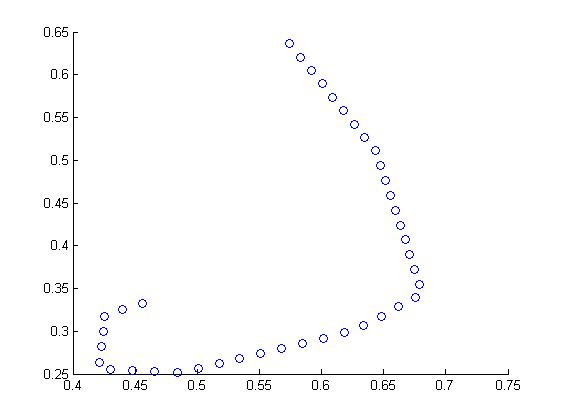
\includegraphics[width=0.2\textwidth]{./figures/letter_before_preprocessing}
        }
        \subfloat[]{
           \label{fig:letter_after_preprocessing}
           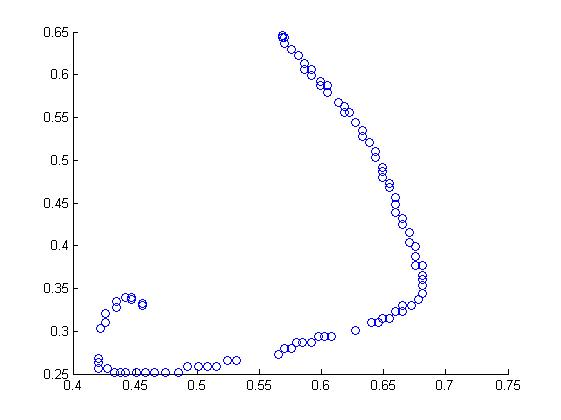
\includegraphics[width=0.2\textwidth]{./figures/letter_after_preprocessing}
        }        
    \caption{The letter \RL{d} before (a) and after (b) preprocessing}
   \label{fig:D_before_after_preprocessing}
\end{figure}

\subsubsection{Horizontal Fragment identification}
The goal of this process is to identify HF's in the written text. Once an HF is detected, its medial point is marked as a candidate point (CP). A HF a subsequence of the stroke having the following properties: 
\begin{enumerate}
\item relatively straight (has low complexity measure)
\item low slope
\item directed right to left 
\end{enumerate}
The method described below tries to identify the largest possible HF and disregard small horizontal regions that are usually caused by the imperfection of the digitizer. The horizontal fragment is performed by spotting the start and the end point of the horizontal fragment. For every newly obtained point, the slope is calculated.\\

The process is ongoing thus to get the largest possible HF, we mark both the beginning and the end of the horizontal segment, these two points were given the names "start horizontal Fragment" (SHF) and "end horizontal Fragment" (EHF). 
A point $p_{i}$ is named a "horizontal point" if the slope of the line $\overline{p_{i-1}p_{i}}$ if $\frac{\Delta x}{\Delta y}\leq0.6$ i.e the angle between the HP and the positive x-axis $\phi \leq \frac{\pi}{6}$ . This parameter was tunes empirically. The same exact value for this parameter was found independently in \cite{daifallah2009recognition} which strengthen our confidence in the finding.\\
To reliably calculate the slope value, despite the noisy data obtained by the tablet, some preprocessing steps need to be performed. However a whole process of normalization, simplification and re-sampling mentioned in the previous may be costly. Since this preprocessing need to be performed on almost every newly obtained point, it would be impractical and can't be performed on-line while the stroke is being written.\\

The preprocessing include only down-sampling of the trajectory, to the half of the sample points of the original trajectory.
Once a low slope point is recognized, the algorithm sets this point as a HF starting point. Every next low slope point is marked as "Last Seem Horizontal point" Until a high slope point is obtained. The point lastly marked as "Last Seen Horizontal point" is set to be an "Ending Horizontal point".\\

Ideally the whole process should be initiated on every new point received by the digitizer, however, it is unnecessary since no much information is obtained by each new point. Alternatively, the process is invoked on every k point, when k is set to 5 in our system. A horizontal fragment must contain two points at least.\\

The nominated segmentation points in this stage is supposed to be an over-segmentation of the stroke. In table \emph{[]} in section \emph{[]} we show that almost all true segmentation points were included in the over-segmentation imposed in this stage. 
It is important the note that this process is imperfect and may result in finding fragments that would not be classified as horizontal segment by a human perform the same task. However, it is important not to apply too many restrictions such imposing too large minimal length on the HF, since while extra CP can be easily filtered out in a later phase when the entire stroke is available, failing to find a CP can't be recovered.\\

\emph{[mention the merge candidate point.]}

% Candidate point types: valid, invalid.
% True segmentation point types:  found, Missed.

\begin{figure}
\centering
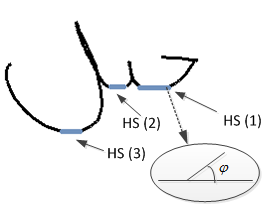
\includegraphics[width=5cm]{./figures/horizontal_segments}
\caption{Horizontal Segments [HS] of the word \RL{jbl}(JABAL)}
\label{fig:horizontal_segments}
\end{figure}

\subsubsection{Sub-strokes scoring}

\begin{figure}
\centering
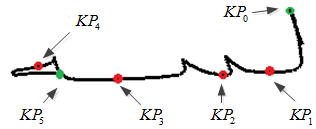
\includegraphics[width=7cm]{./figures/candidate_points}
\caption{Candidate points of the word  \RL{lbyh}. The first and last candidate points are colored in green. The red points are the actual candidate points}
\label{fig:candidate_points}
\end{figure}

Let $CPA$ refer to the array containing the indexes of the candidate segmentation point in the stroke $S$. i.e. $CPA_{i}$ contains the index of the $i^{th}$ CP. Since the first point of the stroke $S$ (i.e. $p_{1}$) is always the beginning of a letter and the last point in the stroke $S$ (i.e. $p_{n}$) is always and last point of a letter, the \emph{Generalized Candidate points array} ($GCPA$) will be a zero based array and will contain two more cells than the $CPA$. Assuming $L$ candidate points were found, below how $GCPA$ is defined: 
\begin{equation}
GCPA_{i} =\begin{cases} 1, & \mbox{if } i=0 \\
							CPA_{i}, & \mbox{if } 1\leq i \leq L \\
							n, & \mbox{if } i=L+1 
			\end{cases}				
\end{equation}
A sub-stroke $S_{i}^{j}$ is a sub-sequence of the stroke $S$ that starts at $GCPA_{i}$ and ends at $GCPA_{j}$ , i.e.
\begin{equation}
S_{i}^{j}=(p_{k})_{k=GCPA_{i}}^{GCPA_{j}}; i<j
\end{equation}
The Sub-sequence Scoring Matrix $D\in\mathbb{R}^{n\times n}$ contains the resemblance scoring obtained by the classifier to the corresponding sub-strokes in$S$, i.e:
\begin{equation}
D(i,j)=Score(S_{i}^{j})
\end{equation}
It is clear that $D$ is an upper triangular matrix. In-order to maintain good performance as well as high segmentation accuracy, we added a locality constraint to avoid marginal segmentation. That is, we only calculate a narrow band of the $D$ matrix above the main diagonal. Assume the band width is equal to $B$.
\begin{equation}
D(i,j)=\inf \Leftrightarrow j \leq i \vee j-i>B 
\end{equation}
Our hypothesis is that sub-strokes that represent a letter will achieve better resemblance scoring, i.e. $D(i,j)$ value will be smaller relative to other sub-stroke. The matrix $D$ is calculated while the stroke is being scribed. Once a new CP is identified, let it be the $j^{th}$ element in the $GCPA_{j}$ a new row and column are added to the matrix $D$. However since the matrix is upper triangular matrix and also the relevant cells are constrained by $B$ width band, the maximal number of cells that will be actually calculated is $B$, all located in the new column. Formally, only the cells $D(k,j)$ which maintain $j-B\leq k \leq j-1$ will be calculated.\\

A letters classifier that is described in depth in \emph{[my paper]} is used to score the sub-strokes. For the sake of completeness, here we will outline the main idea of the classification system. The classifier uses Shape Context to extract the pattern feature, then Earth movers Distance embedding technique descried in \cite{shirdhonkar2008approximate} to project samples of the Arabic letters to a high dimensional $L_{1}$ space. A combination of Principle Component Analysis (PCA) and Linear Discrimination Analysis (LDA) is used to reduce the samples dimensionality and k-NN are found using k-dtree. The exact resemblance score is determined by a minimum score that is given by a predefined linear combination of the $L_{1}$ distance in the embedding space and Sokoe-Chuba DTW.\\

The classifier contains four databases, one for each letter position. It receive a sequence and a position (Ini, Mid, Fin and Iso).
As mentioned earlier a stroke spans from the "mouse-down" to the "mouse-up" event. A stroke that contains a complete WP may contain only the following letters position sequence: \{Iso\} or \{$Ini,Mid^{*},Fin$\}.
However since a stroke could contain a partial WP, the letters of the stroke may have one of the following options, where the  $^{+}$ notation represents more than one occurrence and $^{*}$ notation represents zero or more occurrences.:
\begin{multicols}{2}
\begin{itemize}
    \item $Fin$
    \item $Iso$
    \item $Mid^{+}$
    \item $Ini,Mid^{*},Fin$
    \item $Ini,Mid^{*}$
    \item $Mid^{+},Fin$
\end{itemize}
\end{multicols}
 
In order to maximize performance and accuracy, the system should attempt to look for the letter label in the smallest number of databases. 
To make the following explanation clearer let us define the following: 
Let $S$ be a sequence which contains $L$ candidate points:\\
\textbf{Initial Subsequence.} A sub-sequence $S_1^k$ where $ 1< k \leq L+1$ will be given the name \emph{Initial Subsequence} (IS).\\
\textbf{Medial Subsequence.} A sub-sequence $S_m^k$ where $m \geq 2 \wedge m< k \leq L$ will be name \emph{Medial Subsequence} (MS).\\
\textbf{Final Subsequence.} A sub-sequence $S_k^{L+1}$ where $k \leq 1$ will be referred to as \emph{Final Subsequence} (FS).\\

The $D_p$ matrix below demonstrates the databases in which the system will require the classifier to look into. It is important to note that the $D$ matrix is filled while the stroke is being written, thus the system has no knowledge on how many candidate points the stroke will end up having or when the writer will end the stroke. However the absence of this knowledge does not affect our local decision because the decision only relies on the fact that as long as the writer did not raise the pen every candidate point found does not represent a final letter. Given the definition above below we present 4 types of sub-sequences that were given the names $\alpha$, $\beta$, $\chi$ and $\delta$ which relates the between the cell location in the $D$ matrix and the database that the classifier will look for the best matches.
\begin{itemize}
	\item \textbf{$\alpha$ subsequence:} IS which is not an FS may contain an initial or medial letter only.
	\item \textbf{$\beta$ subsequence:} MS can contain only a medial letter.
	\item \textbf{$\chi$ subsequence:} FS which is not an an IS can contain only a medial or final letter.
	\item \textbf{$\delta$ subsequence:} IS which is also and IS can represent letter in any position.
\end{itemize}

\begin{equation}
D_{p}=
\left( \begin{array}{ccccccc}
\infty 	& \alpha & \alpha & \alpha  & \cdots & \alpha & \delta \\
\infty  & \infty  & \beta   & \beta   & \cdots  & \beta  & \chi    \\
\infty  & \infty  & \infty   & \beta   & \cdots  & \beta  & \chi    \\
\vdots & \vdots & \vdots  & \vdots & \ddots  & \vdots & \vdots \\
\infty  & \infty  & \infty   & \infty   & \cdots  & \beta  & \chi    \\
\infty  & \infty  & \infty   & \infty   & \cdots  & \infty  & \chi    \\
\infty  & \infty  & \infty   & \infty   & \cdots  & \infty  & \infty \end{array} \right)
\label{dp_matrix}
\end{equation}
%
%\setlength\multicolsep{1pt}
%\begin{multicols}{2}
%\begin{itemize}
%    \item[] $\alpha=\{Ini \vee Mid\}$
%    \item[] $\beta=\{Mid\}$
%    \item[] $\chi=\{Mid \vee Fin\}$
%    \item[] $\delta=\{Iso \vee Ini \vee Mid \vee Fin\}$
%\end{itemize}
%\end{multicols}

For each subsequence, the recognition system returns a set of K potential letters candidates, with their resemblance scoring (in our implementation $K=3$). In the current implementation we consider only the candidate with the best (minimal) scoring, however, any function taking into consideration the scoring returned by the classifier for all the candidate can be used to determine the final scoring of the cell.
Figure \ref{substrokes_demo} visually demonstrates the Subsequences that is scored for each cell in matrix $D$.


\begin{figure}
\renewcommand{\arraystretch}{2}
\begin{tabular}{| c |c | c | c| c | c | c |}
\hline
 & $CP_{1}$ & $CP_{2}$ & $CP_{3}$ & $CP_{4}$ & $CP_{5}$ & $CP_{6}$\\ 
\hline
$CP_{1}$
   & N/A
   & \subfloat{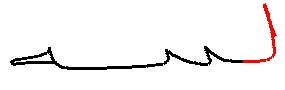
\includegraphics[width=0.8cm]{./figures/substrokes/L}}
   & \subfloat{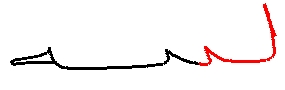
\includegraphics[width=0.8cm]{./figures/substrokes/LB1}}
   & \subfloat{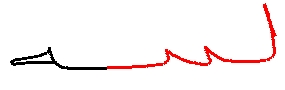
\includegraphics[width=0.8cm]{./figures/substrokes/LB1B2}}
   & N/A & N/A \\
\hline
$CP_{2}$
   & N/A & N/A
   & \subfloat{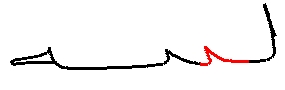
\includegraphics[width=0.8cm]{./figures/substrokes/B1}}
   & \subfloat{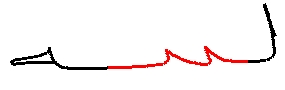
\includegraphics[width=0.8cm]{./figures/substrokes/B1B2}}
   & \subfloat{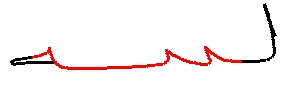
\includegraphics[width=0.8cm]{./figures/substrokes/B1B2H1}}
   & N/A \\
\hline
$CP_{3}$
   & N/A  & N/A & N/A
   & \subfloat{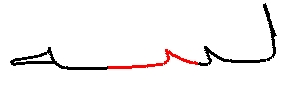
\includegraphics[width=0.8cm]{./figures/substrokes/B2}}
   & \subfloat{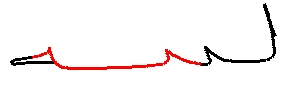
\includegraphics[width=0.8cm]{./figures/substrokes/B2H1}}
   & \subfloat{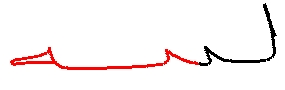
\includegraphics[width=0.8cm]{./figures/substrokes/B2H}} \\
\hline
$CP_{4}$
   & N/A & N/A & N/A & N/A
   & \subfloat{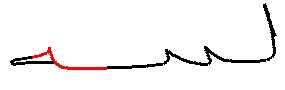
\includegraphics[width=0.8cm]{./figures/substrokes/H1}}
   & \subfloat{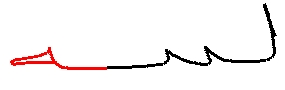
\includegraphics[width=0.8cm]{./figures/substrokes/H}} \\
\hline
$CP_{5}$
   & N/A & N/A & N/A & N/A & N/A
   & \subfloat{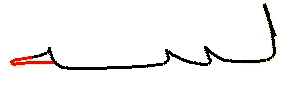
\includegraphics[width=0.8cm]{./figures/substrokes/H2}}\\
\hline
$CP_{6}$
   & N/A & N/A & N/A & N/A & N/A & N/A \\
\hline
\end{tabular}
\caption{Visual demonstration of subsequences of the word shown in figure \ref{fig:candidate_points}}
\label{table:substrokes_demo}
\end{figure}

\subsection{Second  Stage: Candidate points sieving and scoring correction}
In this stage we eliminate redundant segmentation points found in the over-segmentation process found in the previous stage. The elimination is based on the following rules:

\begin{itemize}
	\item [Rule 1]: Inner Segmentation point lies close to the baseline. 
	\item [Rule 2]: Segmentation points do not reside in loops.
	\item [Rule 3]: A sub-stroke length/area is proportional to the stroke/length of the containing stroke.
\end{itemize}

The first is based on the fact that segmentation point lies on the baseline (see []), thus points that are mainly far from the baseline are eliminated. The baseline is proved to be an important piece of information in both segmentation and recognition domains of both on-line and off-line handwriting recognition. In words recognition, it plays a role in determining if an additional stroke to differentiate between diacritic dots according to their position from the baseline (above or under).
The second rule is clear since in most writing styles, segmentation point do not reside inside a loop.
The third rule's goal is to avoid high scoring resulted for discordant scaling of the letters; a scoring correction should be employed. It aims to reduce the effect of scaling problem. To illustrate the discordant scaling problem, see figure below. The suffix of the letter \RL{d} is very similar to the letter \RL{-a}. The only way to visually discriminate between them is by comparing the scaling of this suffix to the whole stroke dimensions. Thus this phase refines the recognition results according the subsequence scale in accordance to the sequence scale. We have penalized sub-strokes that are disproportional to the stroke size by multiplying the score of each sub-stroke with a Gaussian normalized by the stroke area/Length.
In some cases candidate segmentation points are incorrectly nominated on areas that are not horizontal, this is caused from the fact that the nomination is done while the word is being scribed, and our filtering algorithm should be corrected to handle this case.

\emph{[Talk about the scoring correction procedure]}.

\begin{figure}
\centering
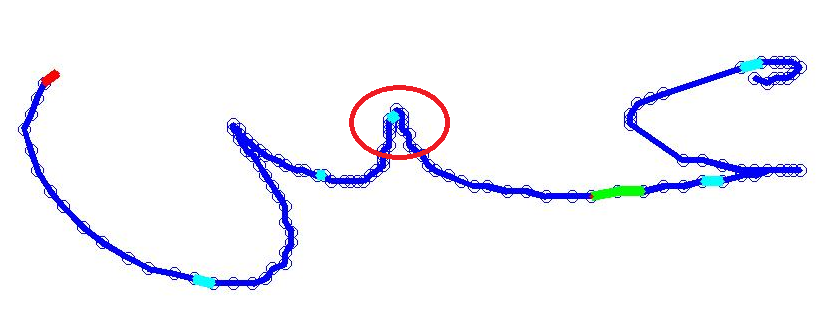
\includegraphics[width=6cm]{./figures/candidate_in_no_horizontal}
\caption{The main body of Arabic word \RL{`yn}. CPs are colored in cyan, Segmentation points are colored in red, a the green areas ensigns that CPs merge has taken place. Three types of false candidate points can be seen: 1. CP on the HF of the letter \RL{-`}. 2. A candidate point that do not reside on a HF. 3. A CP on the valley of the letter \RL{-n}. }
\label{fig:candidate_in_no_horizontal}
\end{figure}

In several cases we encountered candidate points that reside on the same horizontal fragment. [why does it happen?]. We filter out this redundant candidate points in the nomination process and do not wait till this filtering phase. The reason is that since we calculate a narrow band of the Scoring matrix, leaving the impermissible candidate points will result in low performance since highly over segment the word will cause also the system to miss letters because we calculate only a portion a narrow band of the scoring matrix. If such case is identified by the nomination algorithm the medial point between the adjacent candidate points is taken.

\subsubsection{Baseline detection}
Once the entire stroke is available, a baseline detection algorithm is activated only if more than four CP's were detected. The reason for this threshold is to prevent the baseline detection procedure to be activated on small strokes where the baseline can't be reliably determined. To find the handwritten stroke's baseline, the vertical density histogram of the re-sampled stroke is used. The $\Delta y$ of the stroke is calculated and partitioned to 10 intervals, then the center of the of the most common interval is calculated $I_{max}$. A candidate point $CP$ is filtered out if the following holds:
\begin{equation}
|Y(CP)-I_max|>2*max(|I|,0.15) 
\end{equation}
Where $Y(\cdot)$ is the y coordinate of the CP and $|I|$ is the length of the interval. 
Filtering out CPs that are relatively far from the baseline has proven to be very effective in eliminating false CP's that reside on valleys of several letters, such as \RL{q}, \RL{s} and \RL{n}, in the their final and isolated positions. These CPs are usually challenging because they tend to be included in the final set of candidate points if not filtered out. An example can be seen in figure \ref{fig:candidate_in_no_horizontal}, note the candidate point (cyan) inside the last letter \RL{-n}. 

\subsection{Third  Stage: Segmentation Selection}
The goal of this phase is to select the best segmentation points set among the candidate segmentation points. It is done by finding the best segmentation path in $D$ which represent the final segmentation. 
 
A path with the length in the scoring matrix $D^{m\times n}$ is defined as follows:  
\begin{enumerate}
\item First link: $p_{1}=(1,j)$
\item $p_{k}=(i,j)\Rightarrow p_{k+1}=(j,r);s.t.:r>j \forall 1<k<l $
\item Last link: $p_{l}=(1,n)$
\end{enumerate}
Three algorithms are proposed in this work. The first was given the name "Forward Segmentation Selection" (FSS) and the other is was named the “Backward Segmentation Selection” (BSS) and the third named “Greedy Segmentation Selection” (GSS). The final segmentation is the segmentation that has the minimal between the FSS and BSS and GSS normalized by the number of Segmentation points. In the algorithm below, is the set of candidate points Including the pen-down point.  

%\begin{figure}
%\begin{algorithmic}
%$i=1$
%$sum=0$
%\WHILE{$i<|CS|$}
%$j = \mathop {\arg \min }\limits_k \left( {D\left( {i,k} \right)} \right)$
%$FSS = FSS \cup \left\{ j \right\}$
%$sum = sum + D\left( {i,j} \right)$
%$i=j$
%\ENDWHILE
%\end{algorithmic}
%\caption{Forward Segmentation Selection (FSS)}
%\end{figure}

\begin{algorithm}
$i=1$\;
$sum=0$\;
\While{$i<|CS|$}
{
	$j = \mathop {\arg \min }\limits_k \left( {D\left( {i,k} \right)} \right)$\;
	$FSS = FSS \cup \left\{ j \right\}$\;
	$sum = sum + D\left( {i,j} \right)$\;
	$i=j$\;
}
\caption{Forward Segmentation Selection (FSS)}
\label{alg:fss}
\end{algorithm}


%\begin{figure}
%\begin{algorithmic}
%$j={CS|}$
%$sum=0$
%\WHILE{$i<|CS|$}
%$j = \mathop {\arg \min }\limits_k \left( {D\left( {k,j} \right)} \right)$
%$BSS = BSS \cup \left\{ i \right\}$
%$sum = sum + D\left( {i,j} \right)$
%$j=i$
%\ENDWHILE
%\end{algorithmic}
%\caption{Backward Segmentation Selection (BSS)}
%\label{alg:bss}
%\end{figure}

\begin{algorithm}
$j={|CS|}$\;
$sum=0$\;
\While{$i<|CS|$}
{
	$j = \mathop {\arg \min }\limits_k \left( {D\left( {k,j} \right)} \right)$\;
	$BSS = BSS \cup \left\{ i \right\}$\;
	$sum = sum + D\left( {i,j} \right)$\;
	$j=i$\;
}
\caption{Backward Segmentation Selection (BSS)}
\label{alg:bss}
\end{algorithm}

The idea in the following algorithm, is that in each iteration two segmentation point are selected, the first is the best score candidate point from the end of the stroke and the second is the best from the beginning. In this approach, it is less likely to step over segmentation point, like what happened in the FSS and BSS.

\begin{algorithm}
$p_{a}=1$\;
$p_{b}=|CS|$\;
$sum=0$\;
$SSP=\{p_{a},p_{b}\}$\;
\While{$SP \neq \emptyset$}
{
	$p_{a,next} = \mathop {\arg \min}\limits_k (D(p_{a,next},k))$\;
	$SSP = SSP \cup \{p_{a,next}\}$\;
	$sum = sum + D(p_a,p_{a,next})$\;
	Remove all cells that represent a candidate point that has an index lower than $p_{a,next}$\;
	$p_{a}=p_{a,next}$\;
	$p_{b,next} = \mathop {\arg \min}\limits_k (D(k,p_{b,next}))$\;
	$SSP = SSP \cup \{p_{b,next}\}$\;
	$sum = sum + D(p_{b,next},p_b)$\;
	Remove all cells that represent a candidate point that has an index larger than  $p_{b,next}$\;
	$p_{b}=p_{b,next}$\;
}
\caption{Backward-Forward Segmentation Selection (BFSS)}
\label{alg:bfss}
\end{algorithm}

%\begin{figure}
%\begin{algorithmic}
%$p_{a}=1$
%$p_{b}=|CS|$
%$sum=0$
%$SSP=\{p_{a},p_{b}\}$
%\WHILE{$SP \neq \emptyset$}
%$p_{a,next} = \mathop {\arg \min}\limits_k (D(p_{a,next},k))$
%$SSP = SSP \cup \{p_{a,next}\}$
%$sum = sum + D(p_a,p_{a,next})$
%Remove all cells that represent a candidate point that has an index lower than $p_{a,next}$
%$p_{a}=p_{a,next}$
%$p_{b,next} = \mathop {\arg \min}\limits_k (D(k,p_{b,next}))$
%$SSP = SSP \cup \{p_{b,next}\}$
%$sum = sum + D(p_{b,next},p_b)$
%Remove all cells that represent a candidate point that has an index larger than  $p_{b,next}$
%$p_{b}=p_{b,next}$
%\ENDWHILE
%\end{algorithmic}
%\caption{Backward-Forward Segmentation Selection (BFSS)}
%\label{alg:bfss}
%\end{figure}

\begin{algorithm}
$i={1}$\;
$SP=\emptyset$\;
\While{$SP \neq \emptyset$}
{
	$p_{a,next} = \mathop {\arg \min}\limits_k (D(i.j))$\;
	$SSP = SSP \cup \{s,e\}$\;
	$sum = sum + D(s,e)$\;
	Remove all cells that represent a candidate point between $CP_{i}$ and $CP_{j}$\;
}
\caption{Greedy Segmentation Selection (GSS)}
\label{alg:gss}
\end{algorithm}

%\begin{figure}
%\begin{algorithmic}
%$i={1}$
%$SP=\emptyset$
%\WHILE{$SP \neq \emptyset$}
%$p_{a,next} = \mathop {\arg \min}\limits_k (D(i.j))$
%$SSP = SSP \cup \{s,e\}$
%$sum = sum + D(s,e)$
%\STATE	Remove all cells that represent a candidate point between $CP_{i}$ and $CP_{j}$.
%\ENDWHILE
%\end{algorithmic}
%\caption{Greedy Segmentation Selection (GSS)}
%\label{alg:gss}
%\end{figure}

In GSS, in every iteration, the cell with the best scoring is selected thus the selected cell represents a sub-sequence that has the best resemblance for a letter, thus this subsequence must be included in the final segmentation. If cell $D(i,j)$ was selected, both the candidate point $CP_{i}$ and $CP_{j}$ is added to the final set and every segmentation point between $i$ and $j$ are removed from the scoring matrix.

\emph{TODO: show several images of the segmentation process passing through the nomination, the filtering and finally the segmentation selection.}

\section{Validation}
\label{sec:validation}
In similar studies on segmentation, visually inspection take place to validate the segmentation. In this work, we applied an automatic validation process using a ground truth provided by the database. We have used the Subsequence complexity measure (SCM) described subsection \ref{subsec:scm} to automitacally determine if a Final segmentation point is a valid segmentation point (True Positive), i.e. it resides on the same horizontal point the true segmentation point is found, invalid, i.e. it resides on a horizontal segment that is not a real junction point between two connected letters (True Negative) and Missing segmentation points, i.e. the final does not include any point which reside on the same horizontal segment where a true segmentation was supposed to occur there (False Negative).  
For each segmentation point found by our system, for it to be count as a true positive, the information measure between the real segmentation point (marked by an expert human) and the segmentation point sound by the system should be small.

\subsection{Subsequence Complexity measure }
\label{subsec:scm}
The aim of this measure is to give a numerical confidence that if two points reside on the relatively same straight line over the stroke. To demonstrate the idea see figure below. From another point of view, it can be thought about as the amount of information stored in a sub-sequence or the complexity of the sequence. This notion is used in 2 places in our work:
\begin{itemize}
\item The Horizontal fragment identification.
\item In the segmentation point validation step.
\end{itemize}

To calculate the complexity measure of a sequence, first we simplify the subsequence. Then, for each angle  $\phi=\angle(\overline{p_{i-1}p_{i}},\overline{p_{i}p_{i+1}})$ we calculate the parameter $\alpha_{i}$.
\begin{equation}
 \alpha_{i}=\frac{\pi-\theta_{i}}{\frac{\pi}{6}}
\end{equation}
The complexity measure is the defined as:
\begin{equation}
CM(S)=\Sigma_{i}\alpha_{i}
\end{equation}

\begin{figure}[h]
     \begin{center}
        \subfloat[sequence 1]{
            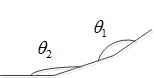
\includegraphics[width=0.2\textwidth]{./figures/angles_1}
        }
        \subfloat[sequence 2]{
           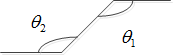
\includegraphics[width=0.2\textwidth]{./figures/angles_2}
        }        
    \end{center}
    \caption{A graphical representation of the angles of a sequence. It can be seen that per our definition Sequence 1 Complexity measure is smaller than sequence 2 complexity measure.}
   \label{fig:sequence_complexity}
\end{figure}

\section{The Database}
\label{sec:database}
The data is the most important part of any supervised learning technique. The data is used for both learning, validation and testing stages and has a critical effect on the system performance. In this work we have chosen to use the ADAB database. The ADAB database is de-facto a standard in the on line Arabic handwriting recognition research field. It is freely available and consists of more than 20k Arabic handwritten words scribed by more than 170 different writers. The words are taken from the 937 Tunisian town/village names. It contains the trajectory information and a plot image of the word trajectory. The ADAB-database v.1 is divided to 3 sets. Details about the number of files, words, characters, and writers are detailed in [6]. Our training and testing set both are taken from this database. 
The information in the ADAB database provides for each word its label and the strokes that were written by the writer, no information relating the strokes to letters or to word parts provided, thus, some work needed to be performed to add this information to the database. This edition is needed for providing letters samples for our classifier as well as for being able to automatically evaluate the segmentation rate. We have created a friendly UI system that reads the samples in the ADAB database, and a human professional segment the samples. The output of this process is an xml for each word sample that contain letter level information, and WPs level details. Since additional strokes are not our interest in the segmentation process, the system automatically filtered out additional strokes. The professional had the ability to filter our additional strokes that could not be identified by the system as such. We have manually segmented ~8k samples which consisted about ~20k strokes.
Our system reads an xml files, extracts the strokes and information we provided our training system with letters and also extracted strokes to test our system. 

\section{Experimental Results}
\label{sec:results}
Our system was implemented in Matlab environment. The total number of samples in the test set is 200. As mentioned a sample is a Tunisian city name, a city name can contain 1 or more words. \\
\emph{it is never easy to compare results of the handwritten recognition or segmentation system with other researches in the literature. The main problem that arise are the different experiment settings and the difference in the experimental methodology, the different experimental setting and the handwriting database.}
Although our approach segments the written script in the stroke level, it is more reasonable to display the results in the WP and word levels. A correct segmentation of a word-part means that all the strokes of the in it were segmented correctly. A correctly segmented stroke is the case when all the letters in the stroke are correctly segmented.  In table 1 below, you can see the length distribution of the Word parts in the test set. By length we mean the number of letters the word part contains.
The segmentation points results were validated automatically, if a word part was recognized correctly that means that the segmentation is correct. For each letter we select the 3 letter and shoe our recognition results based on if one of the candidate letters is the correct letter.

\emph{give more information about the number of segmentation points, the good and bas segmentation points (drill down information). see \cite{al2010development}}
\emph{show images of correctly segmented words.}
\emph{show valid and invalid segmentation points before the last phase.}


\begin{table}[h]
\caption{Segmentation Points Results}
\begin{tabular}{ | c | c | }
  \hline
  Total number of Segmentation point & [] \\
  \hline
  Valid Suggested Point (True Positive) & [] \\
  \hline
  Invalid Suggested Point (False Positive) & []\\
  \hline
  Missing (False Negative) & [] \\
  \hline                                    
   Precision & 95.4\% \\ 
 \hline
  Recall &  95.6\% \\ 
 \hline
  Letters Recognition rate & 87.27\% \\
\hline
\end{tabular}
\centering
\label{table:sp_results} 
\end{table}

If the recognition was incorrect, each segmentation point recognized by the system was validated automatically by making sure that there is no much information between the segmentation ground truth and the segmentation provided by the system.

\begin{table}[h]
\caption{Word-Parts Results}
\begin{tabular}{ | c | c | }
  \hline                     
    Total Number of Word Parts & 197 \\ 
  \hline
  Segmentation Rate &  87.7\% \\ 
 \hline
  Recognition Rate &  70.94\% \\ 
 \hline
  Average Time & 0.64 [sec] \\
\hline
\end{tabular}
\centering
\label{table:wp_results} 
\end{table}

\emph{this table should be removed.}
\begin{table}[h]
\caption{Distribution of WP length}
\begin{tabular}{ | c | c | }
\hline
Number of letters in WP & Num WPs\\
  \hline                     
    1 & 25 \\ 
  \hline
  2 &  171 \\ 
 \hline
  3 & 136 \\ 
 \hline
  4 and more & 91 \\
\hline
\end{tabular}
\centering
\label{table:wp_length_dist} 
\end{table}


\subsection{Analysis}
In this section we will discuss some common cases which were not segmented correctly. In part of these cases we did find solutions and some cases were left for future studies to face. 
\subsubsection{Over-segmentation}
To avoid a candidate point nomination in a horizontal fragment at the beginning of the stroke which is in most cases a false candidate point, we have added the limitation that segmentation point is nominated only if the sub-stroke that spans from the beginning of the stroke to the current point, is complex.

\begin{figure}
\centering
        \subfloat[]{
            \label{fig:letters_same_body_1}
            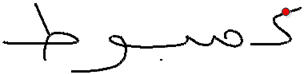
\includegraphics[width=0.3\textwidth]{./figures/oversegmentation_begin_1}
        }
        \subfloat[]{
           \label{fig:letters_same_body_2}
           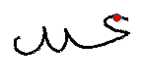
\includegraphics[width=0.15\textwidth]{./figures/oversegmentation_begin_2}
        }        
    \caption{Samples of redundant Candidate point at the beginning of the  stroke.}
   \label{fig:oversegmentation_begin}
\end{figure}

Over segmentation can be caused from typing a letter in a weird form where it is spanned over several strokes. \emph{elaborate and show an image}
%Example: of a letter written in multiple strokes - 1233562203787.xml

\begin{figure}
\centering
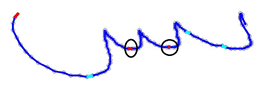
\includegraphics[width=5cm]{./figures/oversegmentation_s}
\caption{Over-segmentation in the letter س. These happens since this letter is very similar to the appearance to a combination of two consequtive ب (ـببـ) letters and only can be identified from the context and using the additional strokes }
\label{fig:oversegmentation_s}
\end{figure}

\begin{figure}
\centering
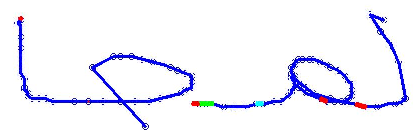
\includegraphics[width=5cm]{./figures/oversegmentation_m}
\caption{Over-segmentation appeared frequently in the letter M, since it contains two horizontal segments (can be handled by eliminatinf candidate points in a loop).}
\label{fig:oversegmentation_m}
\end{figure}

\subsubsection{Under-segmentation}
It may results from 2 reasons:

\begin{enumerate}
\item No point is get nominated in the horizontal fragment
\item Nominated but not selected.
\end{enumerate}

The first mainly results from letter pairs that do not contain horizontal joint between them; this issue is partially solved by extending the notion of a letters to include such pairs of letters. For example the pair لم and لح, these letters may have 2-4 positions. The second may result from nomination of a candidate point on correct horizontal segment but in a late fraction of the segmentation fragment which result is a low scoring and thus not being selected by the Segmentation selection algorithm. This issue usually occurs in the letter و in its final position.

\begin{figure}[h]
\centering
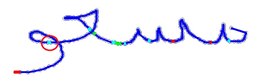
\includegraphics[width=5cm]{./figures/undersegmentation_w}
\caption{An example of a late candidate point in the letter و.}
\label{fig:undersegmentation_w}
\end{figure}


\begin{table}[h]
\caption{Performance of each Segmentation selection algorithm}
\begin{tabular}{ | c | c | c | }
\hline
Segmentation Selection & WP Segmentation & WP Recognition \\
Algorithm & Rate & Rate \\
\hline                 
  FSS & 81.5\% & 70.9\% \\ 
  \hline
  BSS & 78.4\% &  37.5\% \\ 
 \hline
 GSS & 77.1\% & 68.7\% \\ 
 \hline
  FBSS & 83.34\% & 73.74\% \\
\hline
\end{tabular}
\centering
\label{table:ss_algorithms_results} 
\end{table}

\emph{ show statistics of the number of real horizontal segments that was identified by some CP (and mention that almost there were no misses). Also show show what is the percentage of the CP are redundant.}
In \emph{[]} percent of the cases a corresponding candidate point on the same Horizontal fragment as the true segmentation point was  segmentation point nominated. Some correct candidate points were filtered out in the filtering case, however this happened relatively rarely.Most error in the final segmentation is caused by segmentation selection algorithm. That was the reason we have combined several segmentation selection approaches to achieve the best results.
one may assume that the more samples the system is trained on, the better is the recognition results. This is partially true when there are more than two classes, and when the differences between the number of samples per class is gets bigger.
We will show that the maximal number of letters does not affect much the segmentation rate and recognition rate, the graph will convergence after 200 samples per letter. In figure \ref{fig:num_letter_impact} it is clearly evident that there is a point where allowing more samples per class may decrease the accuracy of the system.

\begin{figure}[h]
\centering
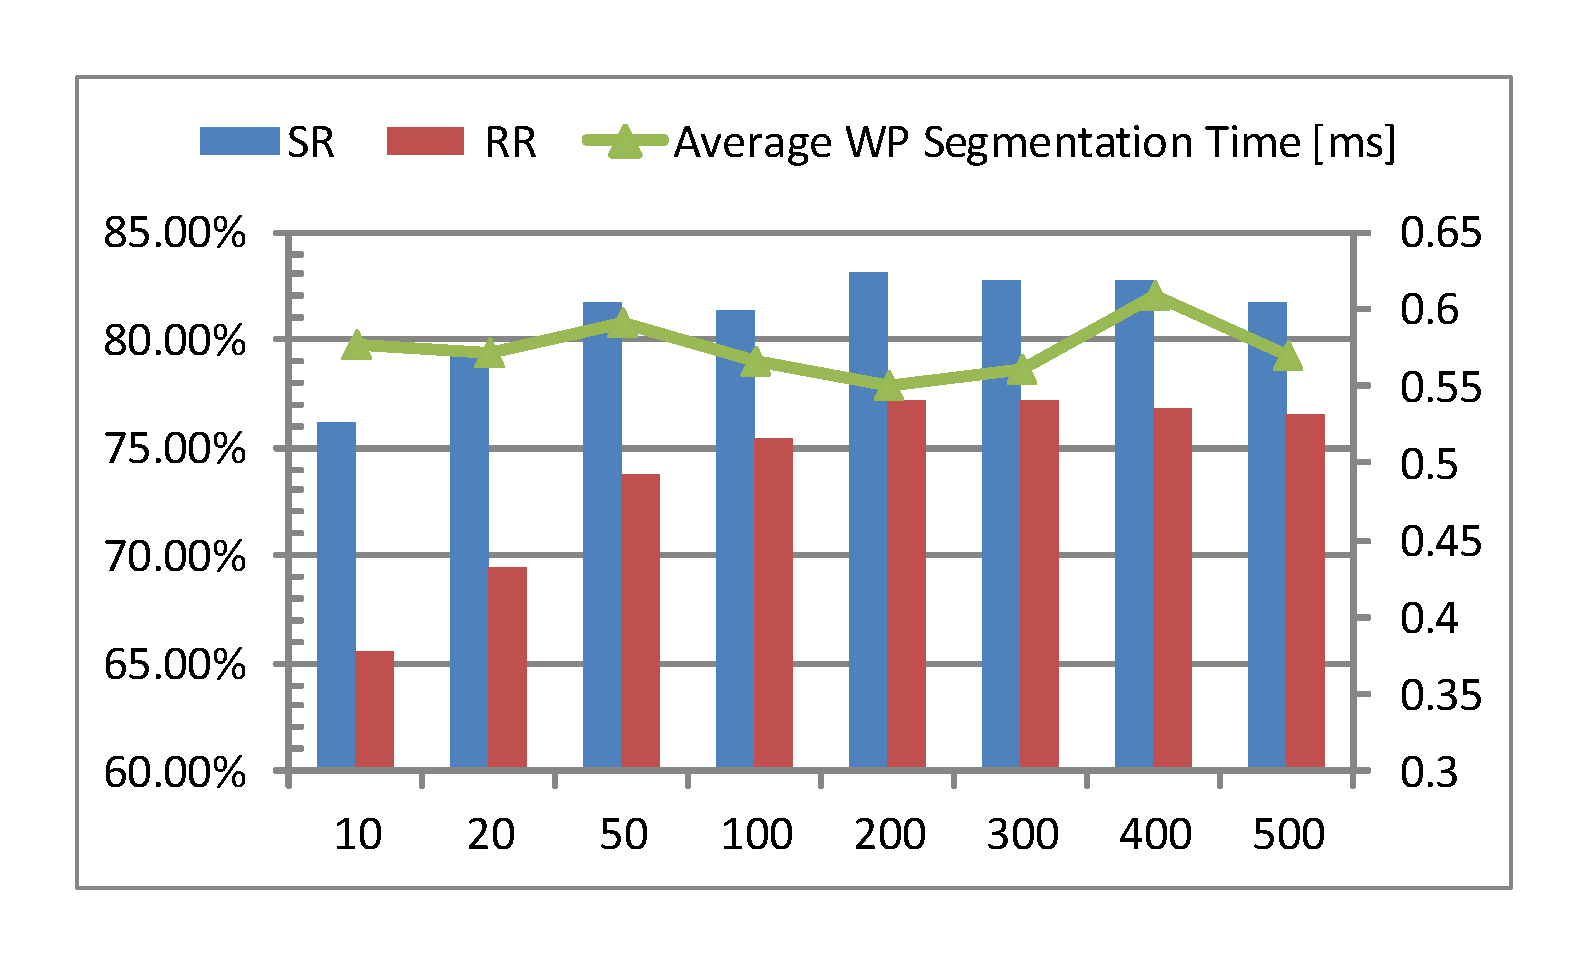
\includegraphics[width=9cm]{./figures/num_letter_impact}
\caption{The diagram shows the influence of the number of letters samples on the segmentation (SR) , recognition rates (RR) , and the average segmentation time. All the three parameters showing convergence when the maximum letter samples per letter position is larger than 200. }
\label{fig:num_letter_impact}
\end{figure}


\section{Future Work}
\label{sec:future_work}
[we can fix the orientation problem in figure work by rotating by different angles but the ADAB sample are our system could easily handle samples to]

[A scoring segmentation point probability techniques can be used to identify the more probable segmentation points]

[Consider the delayed strokes segmentation: every strokes is classified to be in the main body or an additional stroke, id classified in the main body, then we handled it. If classified as a delayed stroke, it should be matched to the letter is related.

For every word, the key a serious of features such that

(A,Ham, KL): أكل
(D,Dot,HB): ذهب


\bibliographystyle{IEEEtran}
\bibliography{IEEEabrv,bibliography}

\end{document}


